\chapter{INTRODUÇÃO}
A crescente complexidade dos ambientes de desenvolvimento e operações de software, impulsionada pela adoção de práticas de DevOps e pela proliferação da computação em nuvem, tem demandado abordagens inovadoras para garantir a segurança das aplicações e da infraestrutura subjacente. No ciclo de desenvolvimento legado, ou tradicional, a segurança era tratada como uma etapa isolada, resultando em atrasos na entrega e em vulnerabilidades detectadas tardiamente.

De acordo com o OWASP Top 10, entre as principais vulnerabilidades do mercado até o ano de 2025 estão a Quebra de Controle de Acesso, Design Inseguro e Configuração Insegura, evidenciando a necessidade de procedimentos e padrões para o estabelecimento de modelos de desenvolvimento ágil e seguro \citeonline{OWASP2025}.

Segundo o relatório IBM Cost of a Data Breach 2024, o custo médio global das violações atingiu os 4,88 milhões de dólares, um aumento significativo em relação aos 4,45 milhões de dólares de 2025 e o maior salto desde a pandemia \citeonline{ibmDataBreachCost}.

Para as empresas do setor financeiro, os custos são ainda mais elevados. As empresas gastam agora 6,08 milhões de dólares a lidar com violações de dados, o que representa um aumento de 22\% em relação à média global.

Nesse contexto, o conceito de DevSecOps emerge como uma evolução do DevOps, integrando práticas de segurança em todas as fases do SDLC, desde o planejamento e design até a implantação e operação \citeonline{kim2021devops}. Simultaneamente, a Infraestrutura como Código (IaC) tem se consolidado como uma prática fundamental para provisionar e gerenciar infraestrutura de forma automatizada e declarativa, utilizando arquivos de configuração versionados \cite{vehent2018securing}.

A sinergia entre DevSecOps e IaC apresenta um potencial significativo para automatizar a integração da segurança na infraestrutura desde sua concepção \citeonline{morris2016infrastructure}. Ao definir a infraestrutura de forma programática, é possível incorporar controles de segurança diretamente nas configurações, garantindo a conformidade e reduzindo a superfície de ataque. A automação propiciada pelo DevSecOps pode então aplicar esses controles de forma consistente e eficiente ao longo do ciclo de vida da infraestrutura.

Com o avanço das práticas de DevOps, a necessidade de integrar segurança como parte essencial do ciclo de desenvolvimento tem se tornado evidente. DevSecOps surge como uma abordagem que incorpora segurança de maneira contínua e automatizada, enquanto Infraestrutura como Código (IaC) oferece meios de gerenciar infraestrutura de forma declarativa e escalável. Esta pesquisa busca unir essas práticas, investigando como elas podem ser integradas para maximizar eficiência e segurança em ambientes computacionais modernos.

\section{Perguntas da Pesquisa}

As perguntas desta pesquisa visam explorar os problemas enfrentados atualmente por empresas e instituições, e elaborar alternativas para contornar ou mitigar estas fraquezas.

A Figura 1 apresenta as principais vulnerabilidades do mercado até o ano de 2025 de acordo com o OWASP Top 10. É possível observar que, entre as principais, estão: Quebra de Controle de Acesso, Design Inseguro e Configuração Insegura.

\begin{figure}[ht]
    \caption{ Riscos críticos de segurança em aplicações web, conforme o OWASP Top 10 de 2025, apresentada em um diagrama que organiza as vulnerabilidades em categorias prioritárias, facilitando a compreensão e a mitigação de ameaças por desenvolvedores e equipes de segurança.}
    \label{fig:owasp}
    \centering
    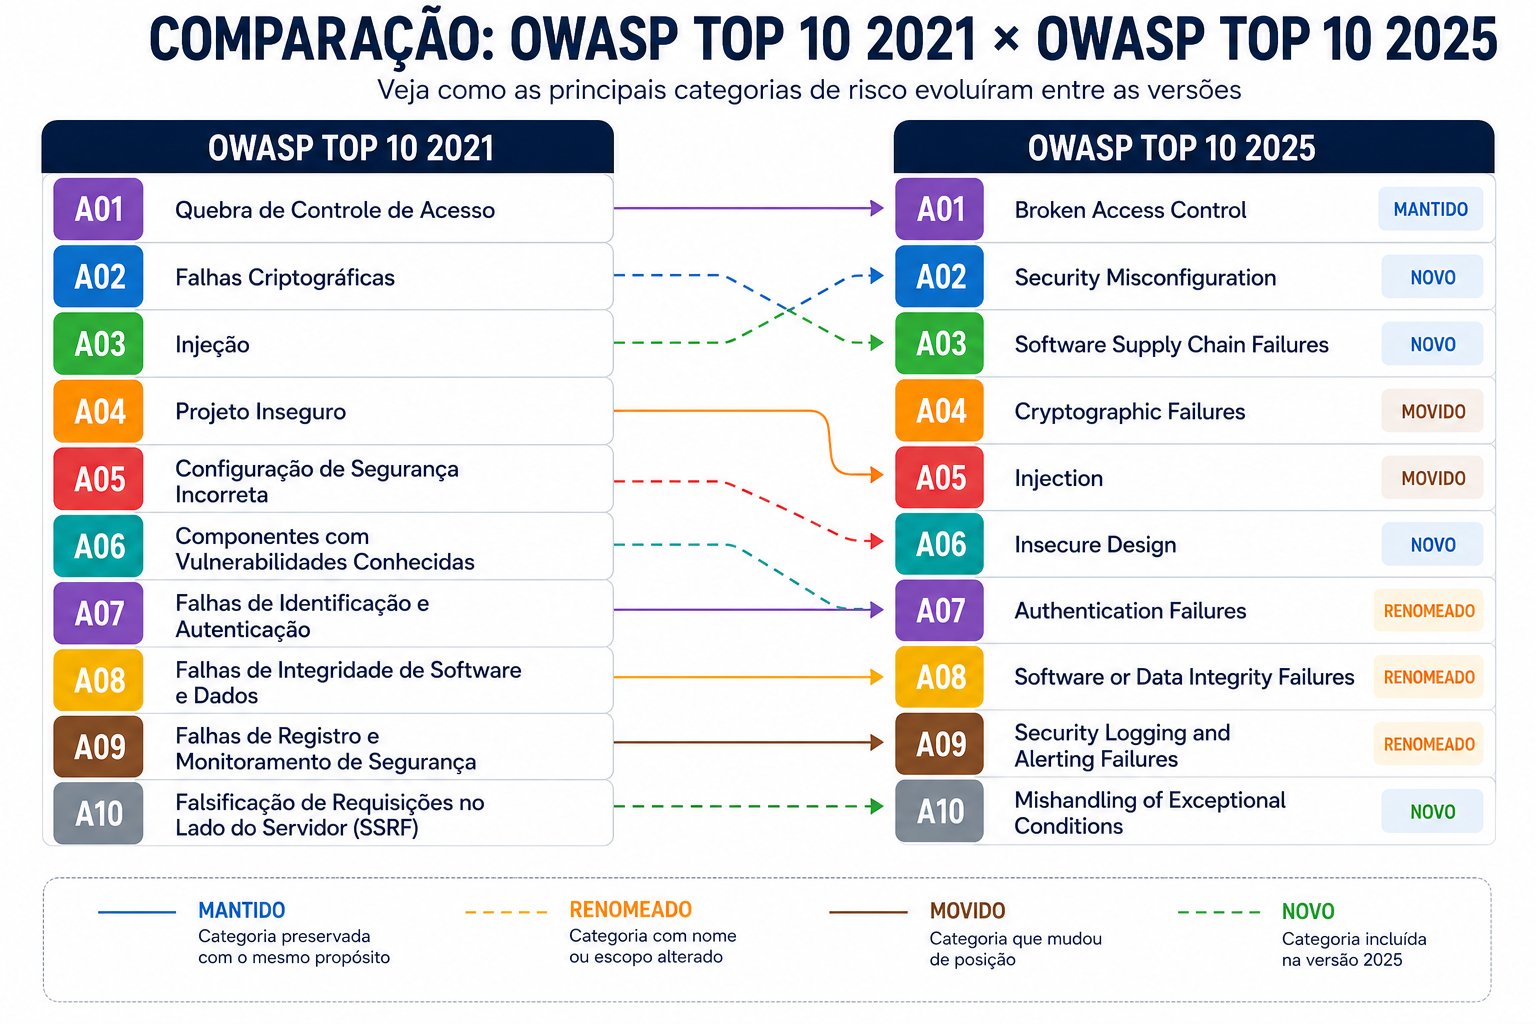
\includegraphics[width=0.8\textwidth]{Arquivos/figuras/Figura_OWASP_Top_10_2025_Diagram.png}
    \fonte{\citeonline{OWASP2025}}
\end{figure}

O OWASP Top 10 é uma lista criada pela Open Web Application Security Project (OWASP) que identifica as dez principais vulnerabilidades de segurança em aplicações web, baseada em dados coletados globalmente. Atualizado periodicamente, o OWASP Top 10 serve como um guia prático para desenvolvedores, arquitetos e equipes de segurança para compreender, priorizar e mitigar os riscos mais críticos. Entre as categorias incluem-se falhas como controle inadequado de acesso, injeção de código (como SQL Injection), exposições de dados sensíveis e falhas na autenticação. Cada item da lista inclui exemplos, impacto potencial, e orientações sobre como prevenir ou remediar essas vulnerabilidades, ajudando organizações a fortalecerem a segurança de suas aplicações e reduzir a superfície de ataque.
    



\begin{itemize}
    \item Como integrar de forma eficaz e automatizada práticas de segurança (DevSecOps) na definição e gestão da infraestrutura por meio de Infraestrutura como Código (IaC), a fim de garantir a segurança e a conformidade desde as fases iniciais do ciclo de vida da infraestrutura?
    \item Como a automação de práticas de segurança (DevSecOps) pode ser integrada na definição e gestão de infraestrutura utilizando Infraestrutura como Código (IaC) para garantir segurança e conformidade desde o início do ciclo de vida da infraestrutura?
    \item Quais são as principais barreiras e desafios para a adoção de práticas DevSecOps no contexto de IaC e como superá-los?
    \item De que forma a integração de ferramentas e processos de DevSecOps com IaC pode melhorar a rastreabilidade, auditabilidade e conformidade em ambientes de infraestrutura complexos?
    \item Quais métricas e indicadores podem ser utilizados para avaliar a eficácia da integração entre DevSecOps e IaC em termos de segurança e desempenho?
    \item Como práticas de DevSecOps baseadas em IaC podem ser escaladas para diferentes níveis de maturidade organizacional e complexidade tecnológica?

\end{itemize}


\section{Justificativa}

 A crescente complexidade dos sistemas computacionais exige abordagens inovadoras para
gerenciar segurança, eficiência e escalabilidade. Esta pesquisa se justifica pela necessidade de reduzir vulnerabilidades e tempo de resposta a incidentes, ao mesmo tempo em que promove práticas de automação. A integração de DevSecOps e IaC tem o potencial de atender a essas demandas de forma sustentável e eficaz utilizando pipelines automatiziados de DevSecOps\footnote{\textbf{Pipeline de DevSecOps:} Fluxo automatizado que incorpora segurança em todas as etapas do desenvolvimento e entrega de software, unindo práticas de DevOps e controles de segurança contínuos.} para tingir estes objetivos.


A integração de DevSecOps e IaC representa uma abordagem promissora para enfrentar os desafios de segurança em ambientes de TI modernos e dinâmicos. A automação da segurança na infraestrutura, desde sua concepção por meio da IaC, pode levar a diversos benefícios, incluindo:
\begin{itemize}
    \item\textbf{Redução de vulnerabilidades:} A incorporação de controles de segurança desde o início do ciclo de vida da infraestrutura diminui a probabilidade de configurações inseguras serem implementadas.
    \item\textbf{Aumento da conformidade:} A automação da aplicação de políticas garante a aderência a padrões de segurança e regulamentações.
    \item\textbf{Melhora na eficiência:} A automação de tarefas de segurança libera equipes para se concentrarem em outras atividades de valor agregado.
    \item\textbf{Redução de custos:} A detecção e correção precoce de problemas de segurança são geralmente mais baratas do que lidar com incidentes em ambientes de produção.
    \item\textbf{Aceleração da entrega:} A integração da segurança no processo de desenvolvimento e implantação da infraestrutura evita atrasos causados por verificações de segurança tardias.
\end{itemize}


A Figura 2 descreve a distribuição de severidade de vulnerabilidades ao longo do tempo, baseada no sistema CVSS, é intrinsecamente ligada às perguntas da pesquisa pois fornece a base visual e quantitativa para investigar a evolução e o impacto das classificações de risco.

O Common Vulnerability Scoring System (CVSS) é um sistema de pontuação que permite classificar a severidade de vulnerabilidades em software e hardware, fornecendo uma medida objetiva do risco associado.
O gráfico apresenta a distribuição da severidade dos riscos ao longo dos anos em três níveis, cada um representado por uma cor: Baixo\text{(Azul)}, Médio\text{(Amarelo)} e Alto\text{(Verde)}.

\begin{figure}[ht]
    \caption{ Distribuição de severidade das vulnerabilidades ao longo do tempo, baseada no sistema CVSS (Common Vulnerability Scoring System), permitindo uma análise visual do impacto e da evolução das classificações de risco em diferentes períodos. }
    \label{fig:cvss}
    \centering
    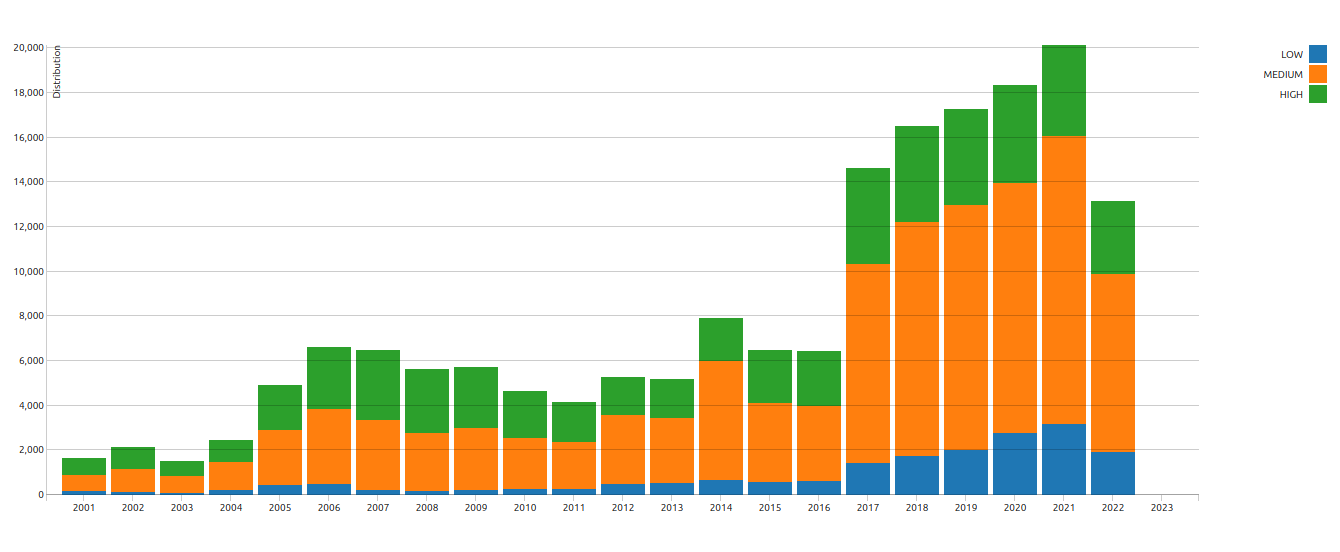
\includegraphics[width=0.8\textwidth]{Arquivos/figuras/Figura_CVSS_Severity_Distribution_Over_Time.png}
    \fonte{\citeonline{NIST2025}}
\end{figure}

A proposição de um modelo de integração claro e prático pode fornecer um guia valioso para organizações que buscam adotar uma abordagem mais proativa e automatizada para a segurança da sua infraestrutura.


\section{Objetivo}
\subsection{Objetivo Geral}

Propor um modelo de integração entre DevSecOps e IaC para automatizar e fortalecer
práticas de segurança em infraestruturas computacionais visando a automação da segurança e da conformidade da infraestrutura ao longo de seu ciclo de vida implementando práticas como \textit{ShiftLeft}\footnote{\textbf{ShiftLeft:}  Estratégia utilizada em DevSecOps que antecipa práticas de segurança no ciclo de desenvolvimento, identificando e corrigindo vulnerabilidades desde as etapas iniciais no ciclo de desenvolvimento de software, reduzindo riscos e custos.}.



\subsection{Objetivos Específicos}

Considerando o desenvolvimento da pesquisa e o objetivo geral apresentado, destacam-se os seguintes objetivos específicos:

\begin{itemize}
	\item Identificar os principais desafios e limitações na integração de DevSecOps e IaC;
	\item Identificar as principais práticas e ferramentas de DevSecOps relevantes para a gestão de infraestrutura;
	\item Investigar as técnicas e métodos para automatizar a aplicação de políticas de segurança e conformidade em ambientes de IaC;
	\item Propor um modelo de integração que detalhe os processos, as responsabilidades e as ferramentas envolvidas na adoção de DevSecOps em IaC;

\end{itemize}

